\documentclass[conference]{IEEEtran}
\IEEEoverridecommandlockouts
% The preceding line is only needed to identify funding in the first footnote. If that is unneeded, please comment it out.
\usepackage{cite}
\usepackage{amsmath,amssymb,amsfonts}
\usepackage{algorithmic}
\usepackage{graphicx}
\usepackage{textcomp}
\usepackage{xcolor}
\usepackage{ctex}
\usepackage{fontspec}
\usepackage{listings}
\usepackage{pxfonts}
% The following code is for matlab language
\lstset{
    columns=fixed,     
    basicstyle = \tt,           % 基本样式 + 小号字体  
    %numbers=left,    % 在左侧显示行号
    frame=none,     % 不显示背景边框
    breaklines = true,                  % 代码过长则换行
    backgroundcolor=\color[RGB]{245,245,244},  % 设定背景颜色
    keywordstyle=\color[RGB]{40,40,255},         % 设定关键字颜色
    % numberstyle=\footnotesize\color{darkgray},    % 设定行号格式
    commentstyle=\it\color[RGB]{0,96,96},         % 设置代码注释的格式
    stringstyle=\rmfamily\slshape\color[RGB]{128,0,0},   % 设置字符串格式
    showstringspaces=false,   % 不显示字符串中的空格
    language=matlab,             % 设置语言
    extendedchars=false,
    %basicstyle=Consolas
    tabsize=4,
    upquote=true,
    %literate={'}{\textquotedb}1
}

\def\BibTeX{{\rm B\kern-.05em{\sc i\kern-.025em b}\kern-.08em
    T\kern-.1667em\lower.7ex\hbox{E}\kern-.125emX}}
\begin{document}

\title{傅立叶变换光谱测量技术实验报告}

\author{
    \IEEEauthorblockN{
        黄润华}
        \IEEEauthorblockA{
            \textit{Ocean University of China} \\
            \textit{email@noreply.com}
    \and
    \IEEEauthorblockN{
        杨超}
        \IEEEauthorblockA{
            \textit{Ocean University of China} \\
            \textit{email@somewhere.com}
        }
    }
}




\maketitle

\begin{abstract}
    本实验报告为傅立叶变换光谱测量技术第五次实验报告,本报告采用Python仿真动镜倾斜误差与采样间隔误差两个因素同时影响下的傅里叶变换光谱测量系统的光谱测量曲线。误差可以是随机、线性或正弦变化的。以632.8nm的HeNe激光和532nm的VAG激光为例为例。采样间隔79.1nm。本仿真以632.8nm的HeNe激光为例。
\end{abstract}

\begin{IEEEkeywords}
    Optical spectrum, python, fft
\end{IEEEkeywords}

\section{实验目的}
\begin{itemize}
    \item[1.] 思考动镜倾斜误差与采样间隔误差两个因素同时影响下的傅里叶变换光谱测量曲线形状;
    \item[2.] 学习掌握Python绘图库基础知识。 
\end{itemize} 

\section{实验原理}
\subsection{单色线的干涉方程}
理论上单色线的干涉图可以用公式(\ref{eq1})来描述
\begin{align}
    I(x) = 2cos(2\pi \sigma_0 x)    \label{eq1}
\end{align}

\subsection{采样间隔误差对干涉方程的影响}
人为进行动镜的平移过程通常掺杂着过程噪声。过程噪声的形式多种多样,常见的简单过程噪声类型为正弦噪声、随机噪声与线性噪声。然而,外部环境是一个不可预测的变量,在不同时刻的噪声类型通常是不相关且随机的,这种随机性带给光谱测量的影响是复杂性的。在操作不当的情况下,动镜移动的距离受到过程噪声的影响较大时,得到的傅立叶变换光谱测量曲线具备较低的可信度同时带来了阅读上的复杂性。

动镜移动时过程噪声带来的采样间隔误差是不可避免的,采样间隔误差的直接影响主要体现在对公式(\ref{eq1})中扫描长度$x$的影响:
\begin{align}
    I(x) = cos(2\pi\sigma_0(x + \varepsilon_s)) \label{eq9}
\end{align}

采样过程通常会选取$2^{12}$到$2^{20}$个采样点,每次采样均有可能存在一定的采样误差,采样误差经过多次迭代后对最终傅立叶光谱测量曲线带来的影响是可观且巨大的。

本次仿真模拟的采样间隔误差均为简单采样间隔误差,即代表每次采样时的误差类型为单一的正弦噪声误差、随机噪声误差或线性噪声误差。同时假设采样过程均为独立事件,前后采样过程噪声互不相干且独立。

正弦形式的采样间隔误差表达式如下:
\begin{align}
    \varepsilon_s = \frac{\lambda_0}{16}sin(2\pi\sigma_{\varepsilon}x)  \label{eq2}
\end{align}
其中波数(Wave number)数值为$\sigma_{\varepsilon} = 0.4\times10^4 m^{-1}$。

随机形式的采样间隔误差表达式可以采用均匀分布来表示:
\begin{align}
    \varepsilon_s \sim U(-\frac{\lambda_0}{5}, \frac{\lambda_0}{5})   \label{eq3}
\end{align}

线性形式的采样间隔误差表达式可以用正比例函数来表示:
\begin{align}
    \varepsilon_s(k) = k, \;\;\; k \in [0, \;79.1\times10^9 m] \label{eq4}
\end{align}

\subsection{动镜倾斜误差对干涉方程的影响}
动镜倾斜误差带来的影响从干涉图上看为在干涉图上添加一个特定的噪声:
\begin{align}
    I = cos(2\pi\sigma_0x) + \varepsilon_m \label{eq5}
\end{align}

本次仿真模拟的动镜倾斜误差均为简单动镜倾斜误差,即代表动镜倾斜误差类型为单一的正弦噪声误差、随机噪声误差或线性噪声误差。

正弦形式的动镜倾斜误差表达式如下:
\begin{align}
    \varepsilon_m = sin(2\pi\frac{\sigma_0}{16}x)  \label{eq6}
\end{align}

随机形式的动镜倾斜误差表达式可以采用均匀分布来表示:
\begin{align}
    \varepsilon_m \sim U(-1, \; 1)   \label{eq7}
\end{align}

线性形式的动镜倾斜误差表达式可以用正比例函数来表示:
\begin{align}
    \varepsilon_m(k) = k, \;\;\; k \in [0, 1] \label{eq8}
\end{align}

\subsection{综合误差对干涉方程的影响}
由式(\ref{eq9})与式(\ref{eq5})可以得到采样干涉误差与动镜倾斜误差两因素同时影响下的干涉图方程:
\begin{align}
    I = cos\left[2\pi\sigma_0(x + \varepsilon_s)\right] + \varepsilon_m    \label{eq11}
\end{align}

\section{实验内容}
仿真动镜倾斜误差因素影响下的傅里叶变换光谱测量系统的光谱测量曲线。误差形式分别为随机误差、线性误差或正弦变化的误差。以632.8nm的HeNe激光和532nm的VAG激光为例。采样间隔选取79.1nm。

\section{实验结果}
本实验报告的分析以632.8nm的波长为例。

\subsection{动镜倾斜误差对光谱曲线的影响}

\begin{figure}[htbp]
	\centerline{
		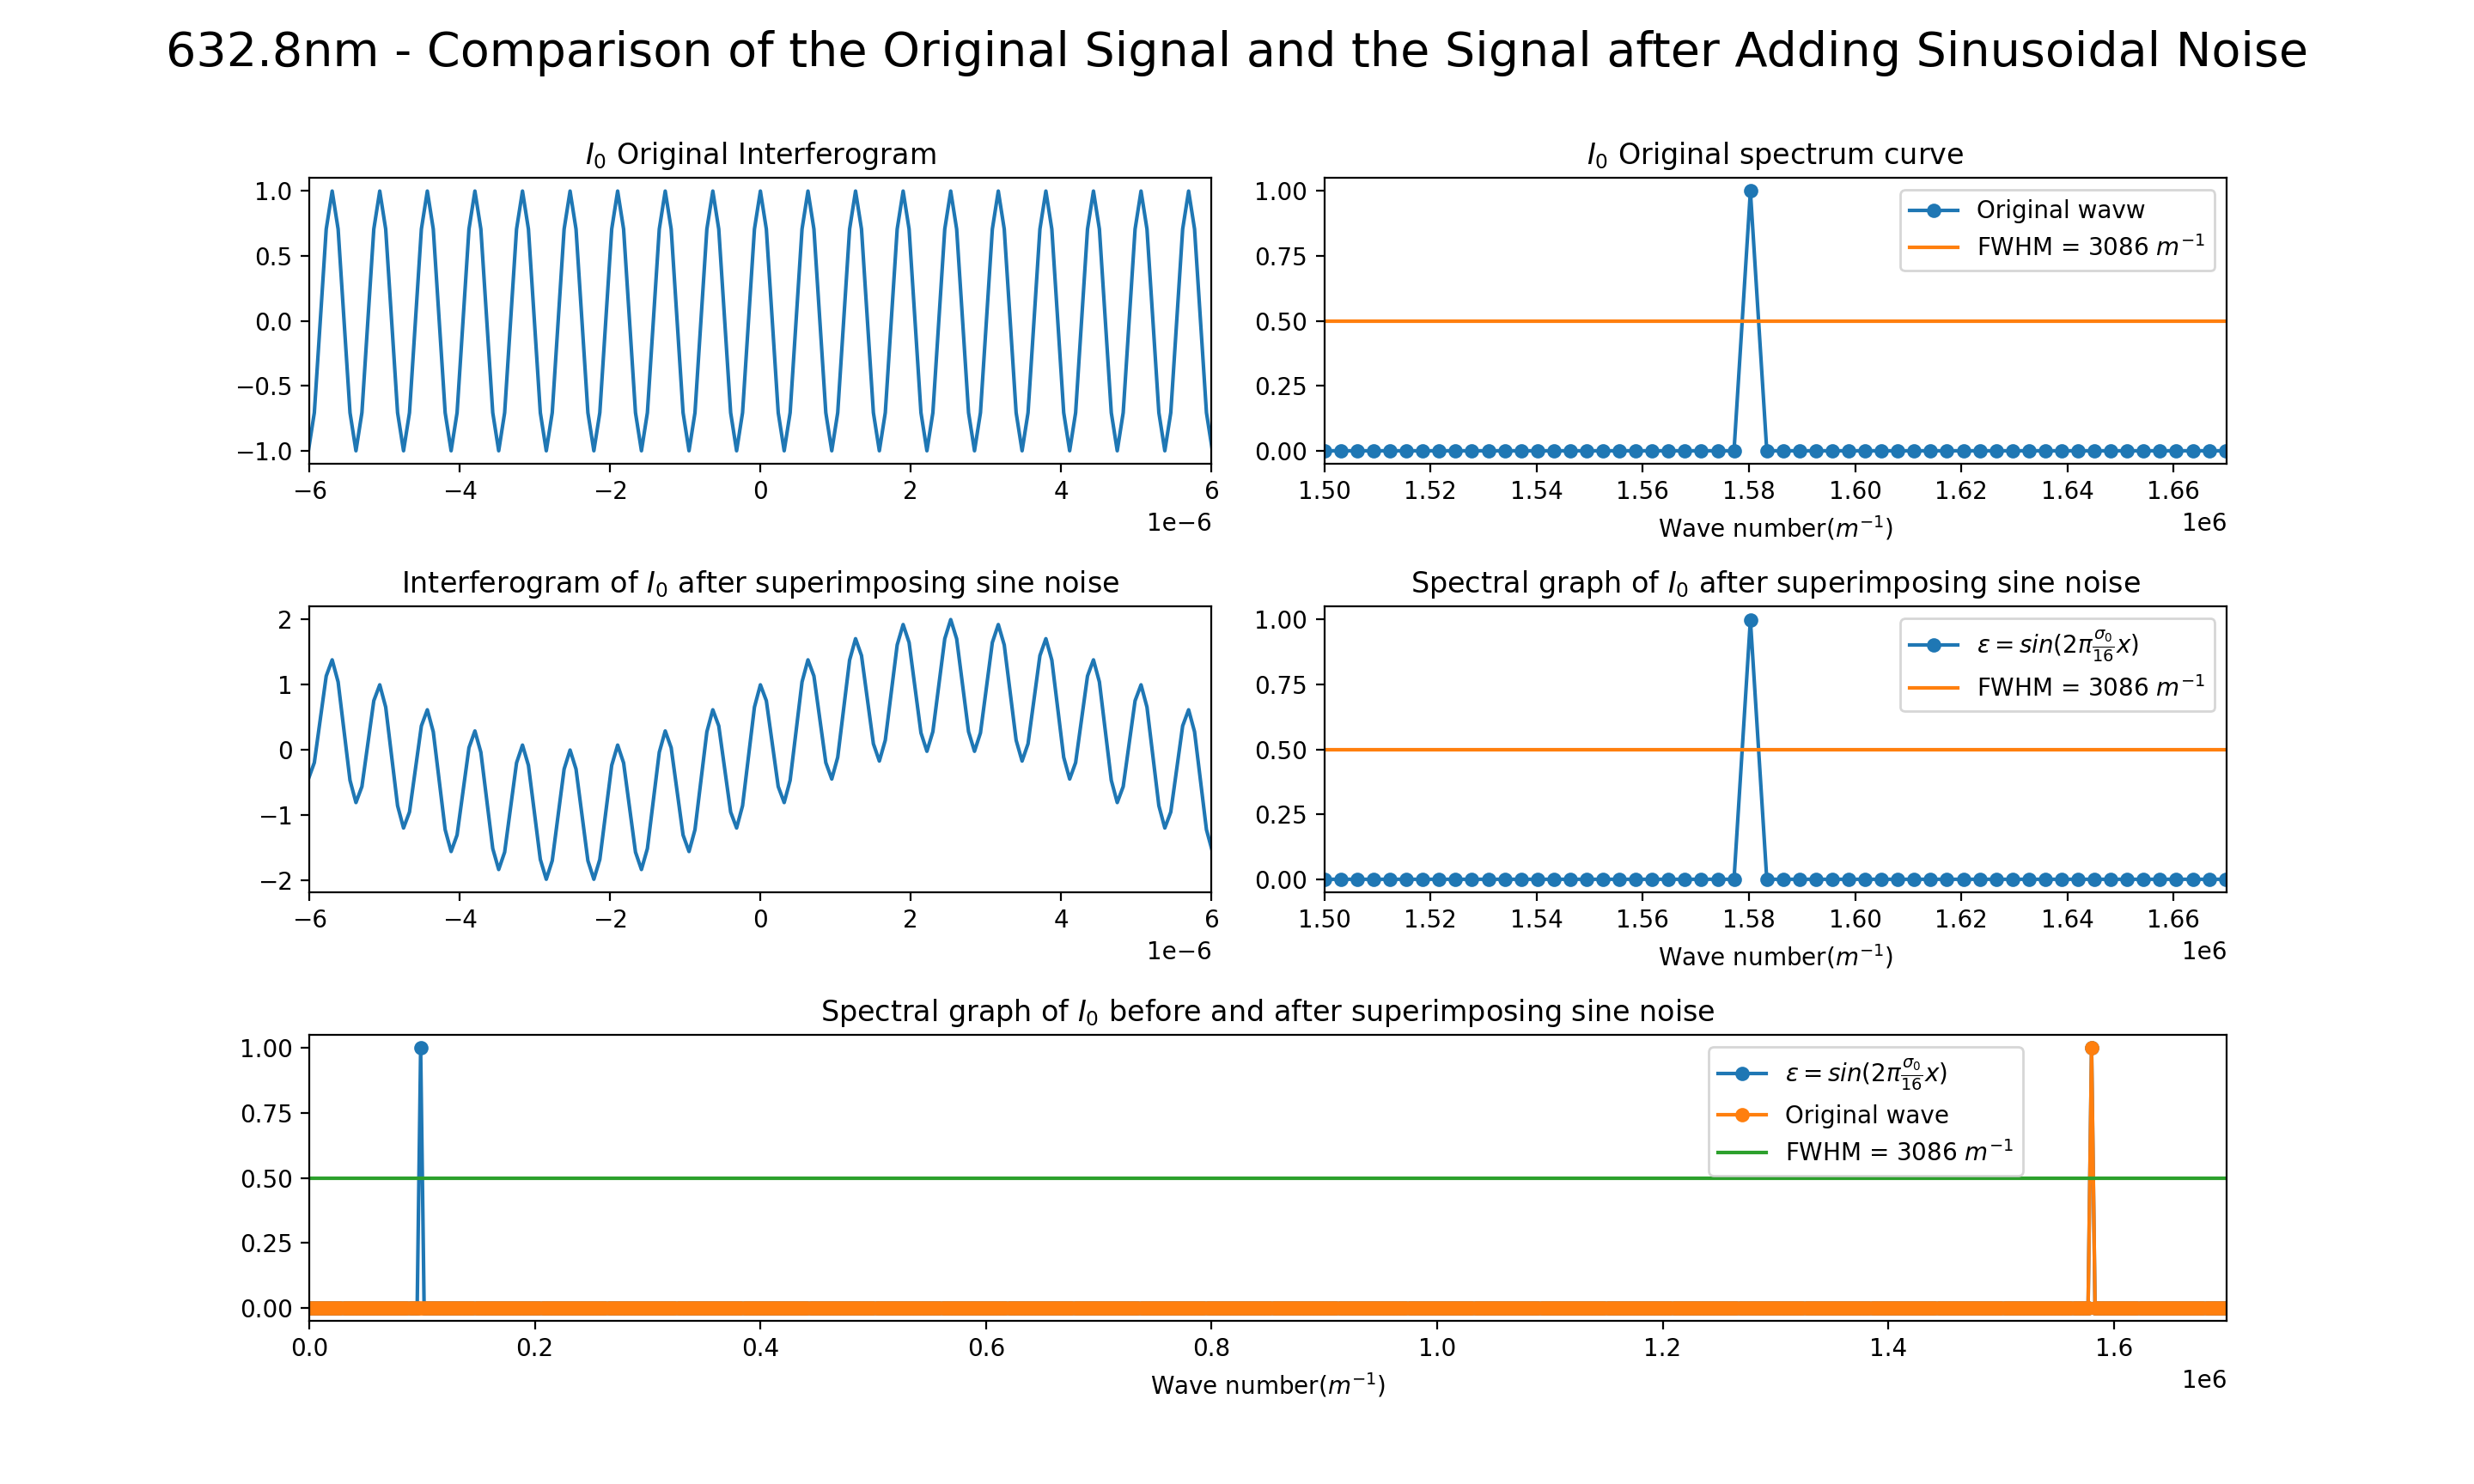
\includegraphics[width=10cm]{1.png} 	
	}
	\caption{正弦形式的动镜倾斜误差对光谱曲线的影响}
	\label{pic1}
\end{figure}

\begin{figure}[htbp]
	\centerline{
		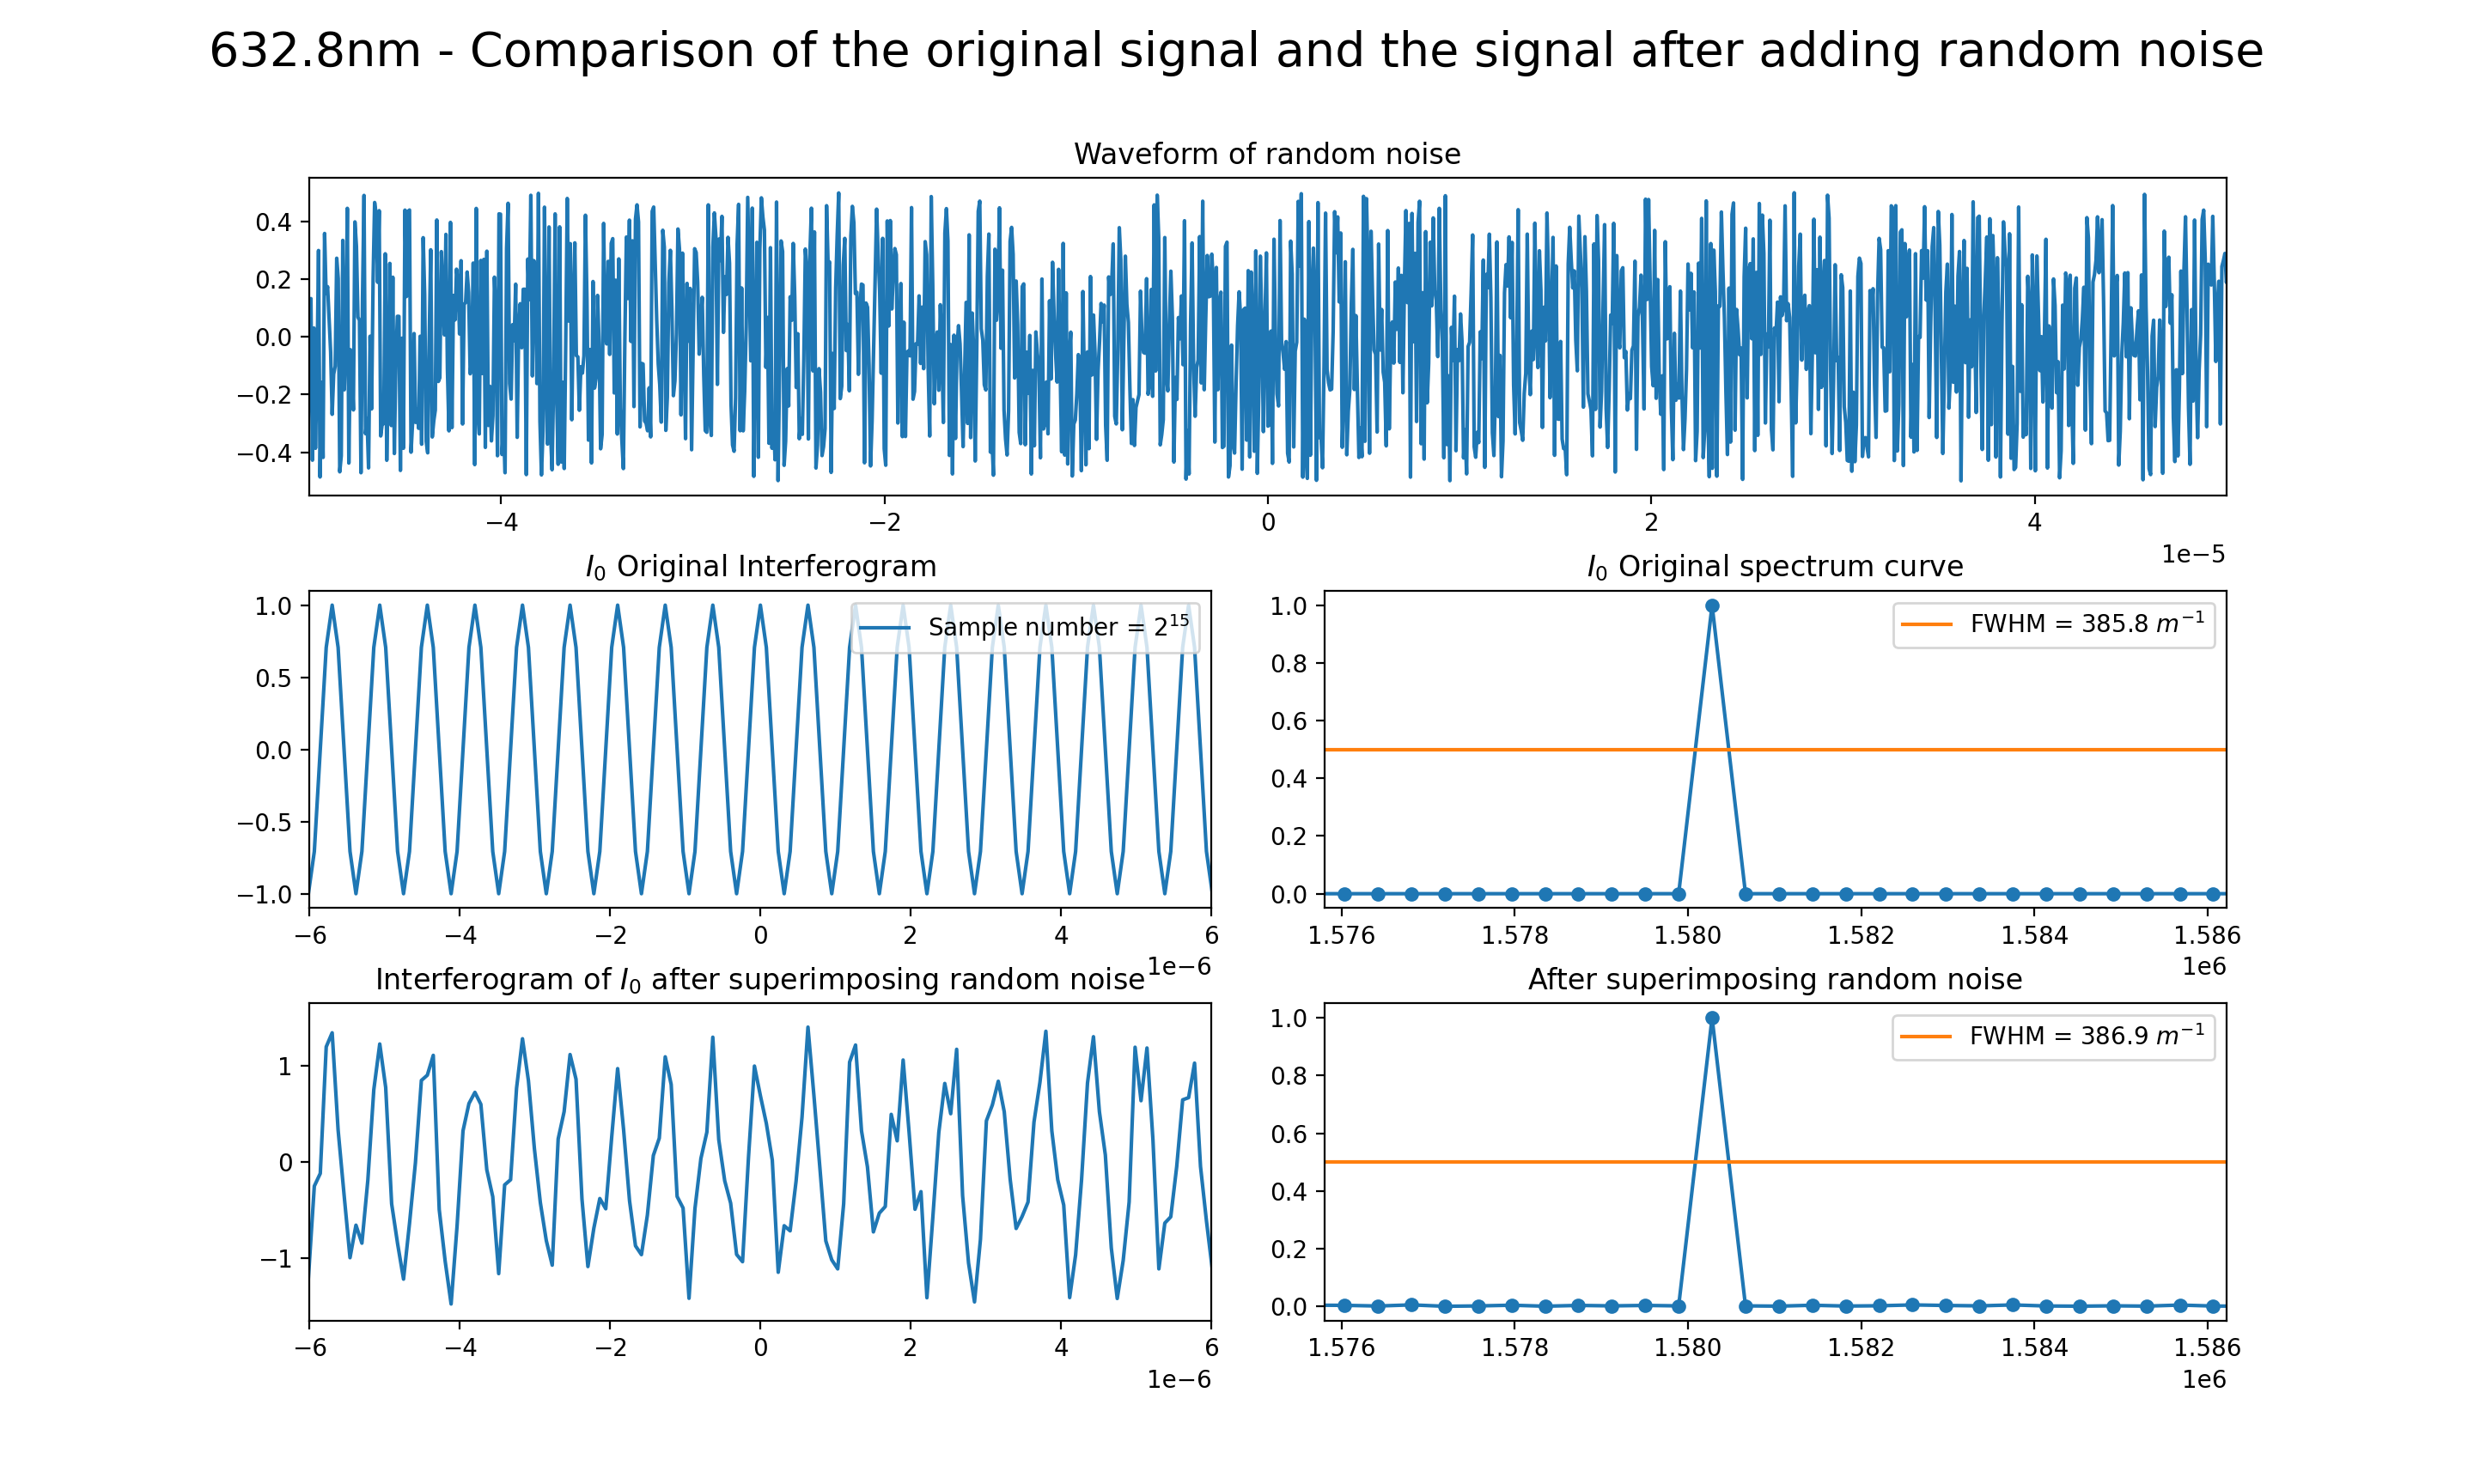
\includegraphics[width=10cm]{2.png} 	
	}
	\caption{随机形式的动镜倾斜误差对光谱曲线的影响}
	\label{pic2}
\end{figure}

\begin{figure}[htbp]
	\centerline{
		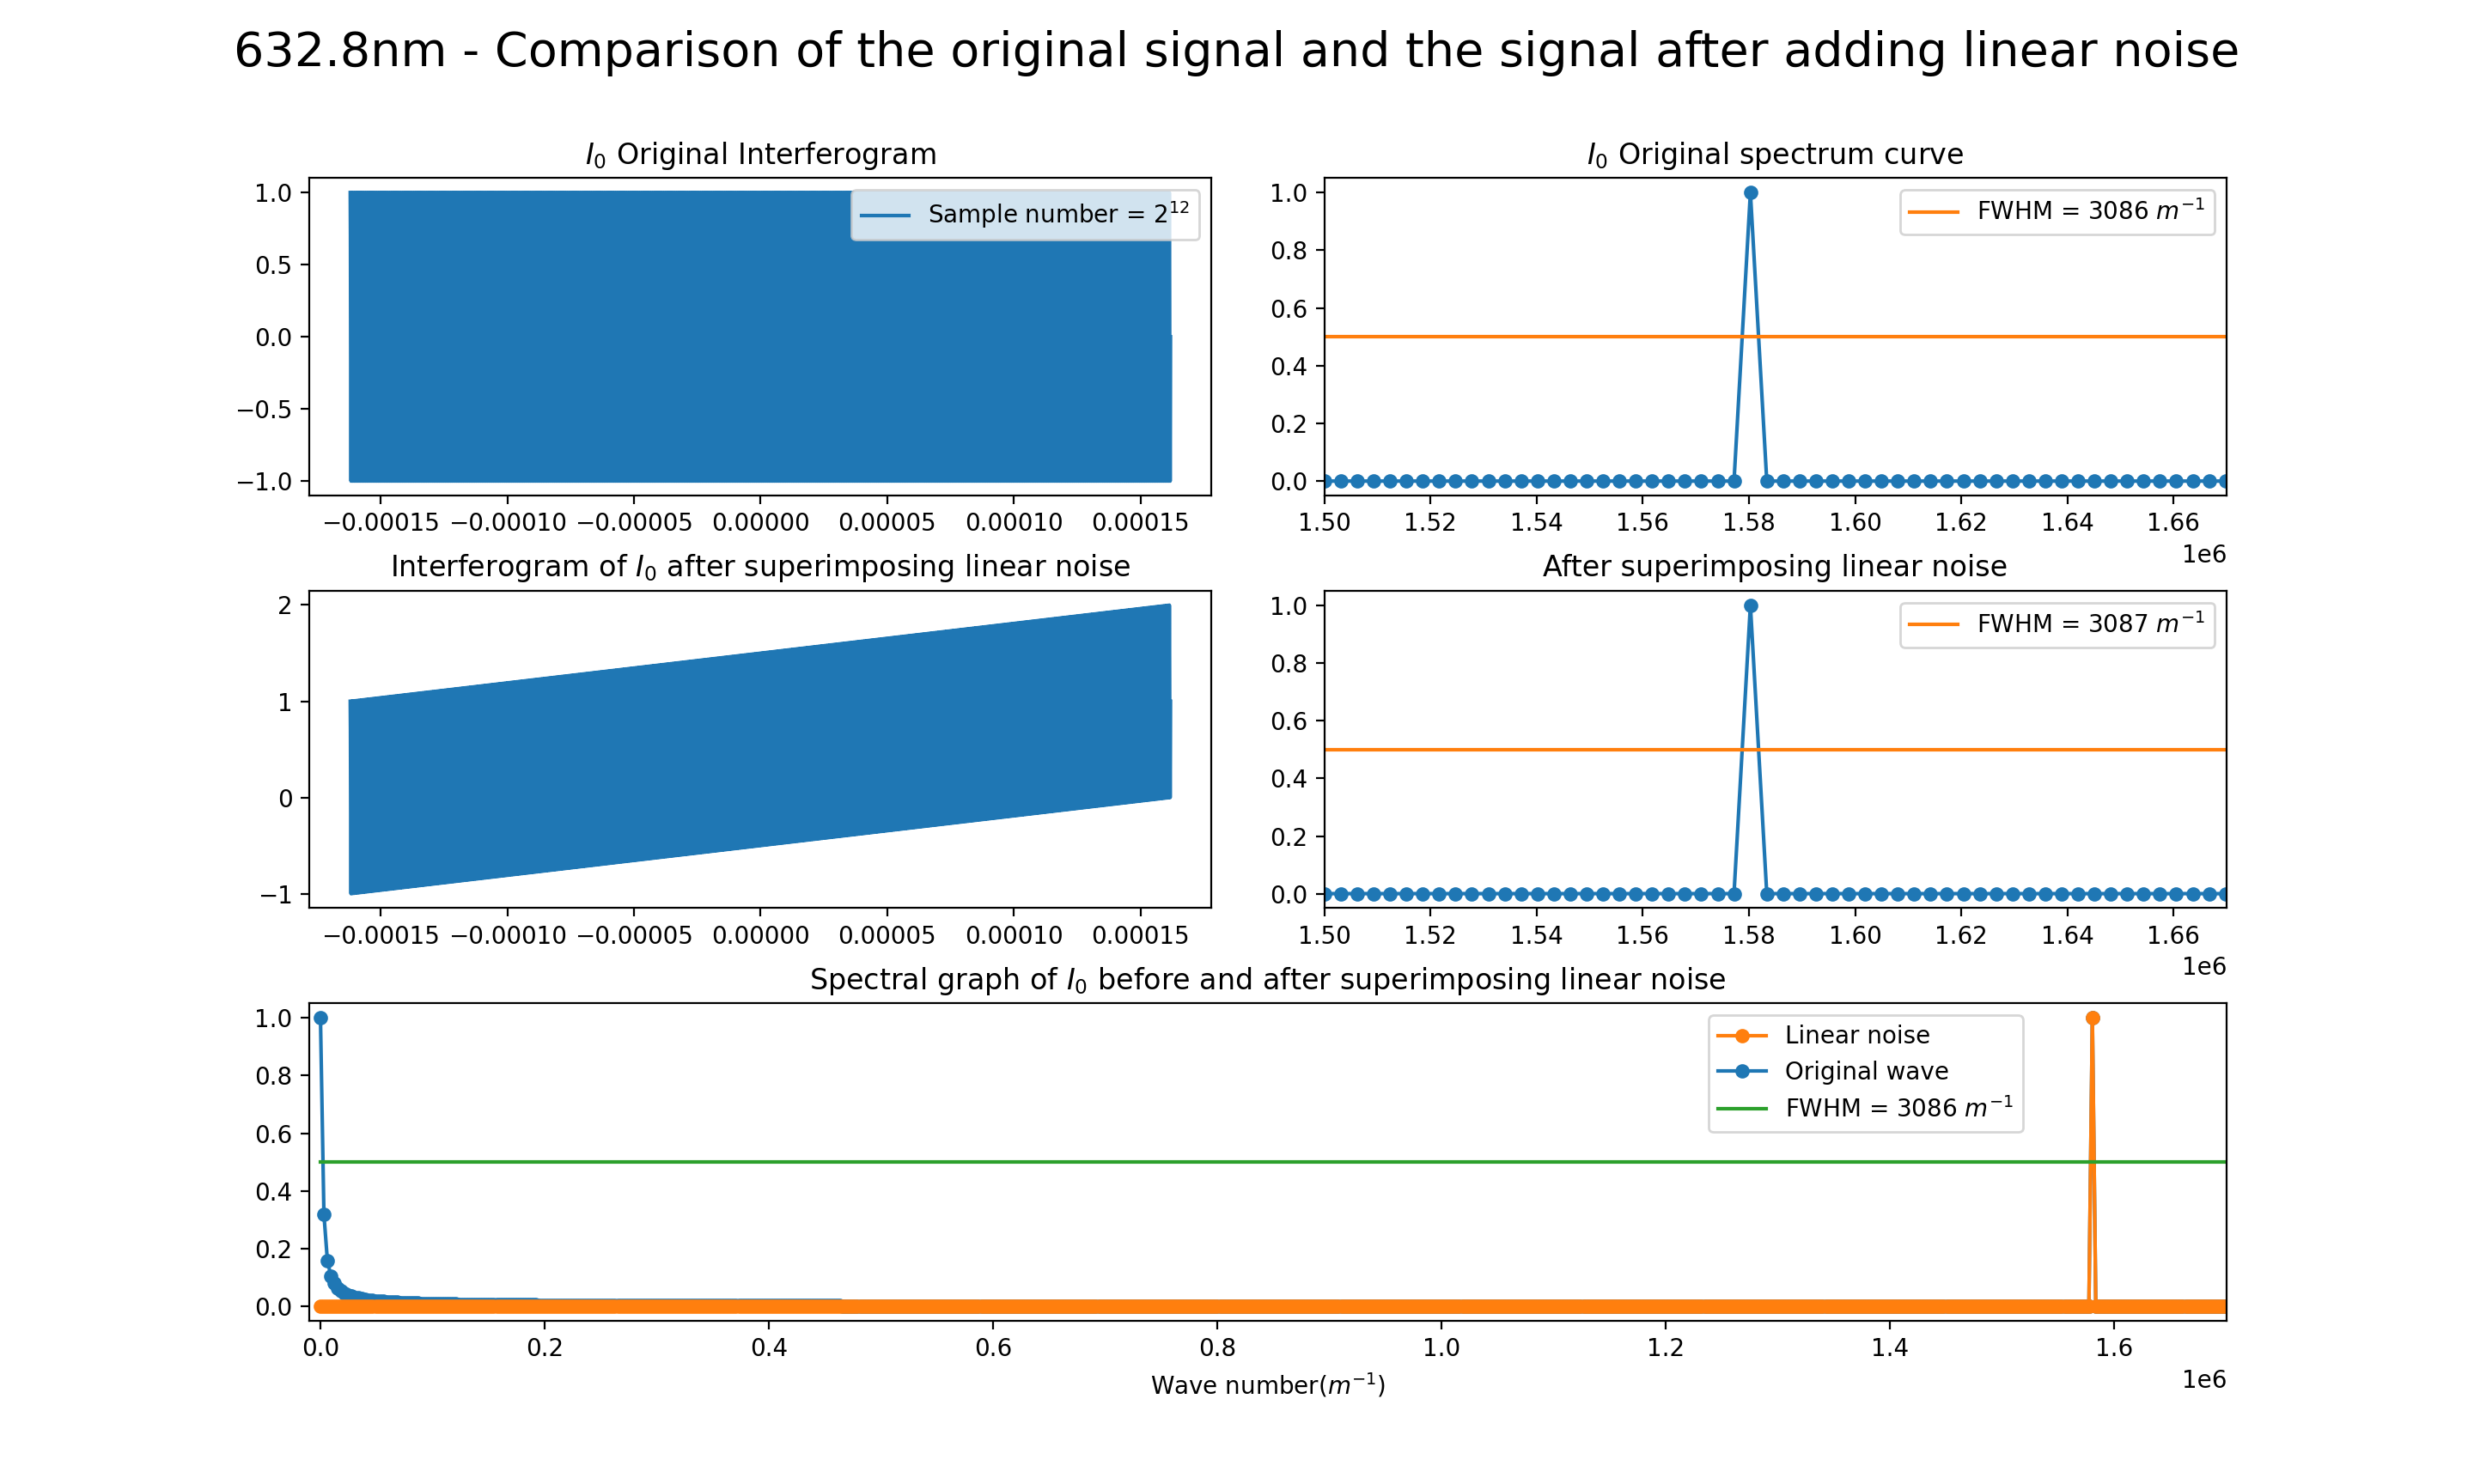
\includegraphics[width=10cm]{3.png} 	
	}
	\caption{线性形式的动镜倾斜误差对光谱曲线的影响}
	\label{pic3}
\end{figure}

图\ref{pic1}、图\ref{pic2}与图\ref{pic3}分别显示了动镜倾斜误差形式为正弦形式、随机形式与线性形式时的干涉图与傅里叶变换后的光谱测量曲线。每张图第一行表示原始未叠加动镜倾斜误差时候的干涉图与傅里叶变换光谱测量曲线,第二行展示了叠加对应的动镜倾斜误差干涉图与傅里叶变换光谱测量曲线,图片第三行为叠加动镜倾斜误差前后傅里叶变换光谱测量曲线的比较。

通过仿真结果可以看出,正弦形式的动镜倾斜误差会使得干涉图整体包络沿着噪声的轨迹变换,同时正弦形式的动镜倾斜误差会在中心波数旁产生一个峰(旁瓣),但对主峰的半峰全宽影响较小,可以忽略不计。

随机形式的动镜倾斜误差对原始干涉图的影响较大,叠加动镜倾斜误差后,干涉图出现参差不齐杂乱无章的现象。由于随机形式的动镜倾斜误差均值为零,因此实际傅立叶变换后的光谱测量曲线在波数为零处没有幅值(即叠加噪声后的干涉图没有直流量)。从图片上进一步分析可以得到随机形式的动镜倾斜误差对傅里叶变换光谱测量曲线主峰的半峰全宽影响较小,但主峰旁的旁瓣出现了毛刺现象。

线性形式的动镜倾斜误差使得原始干涉图的包络按照误差曲线的形式变化。从频谱角度分析,线性形式的动镜倾斜误差对原始单色光主峰的半峰全宽影响较小,可以忽略不计,但由于引入了直流分量使得傅里叶变换光谱测量曲线在主峰附近出现了侧峰。

\subsection{联合误差对光谱曲线的影响}
\begin{figure}[htbp]
	\centerline{
		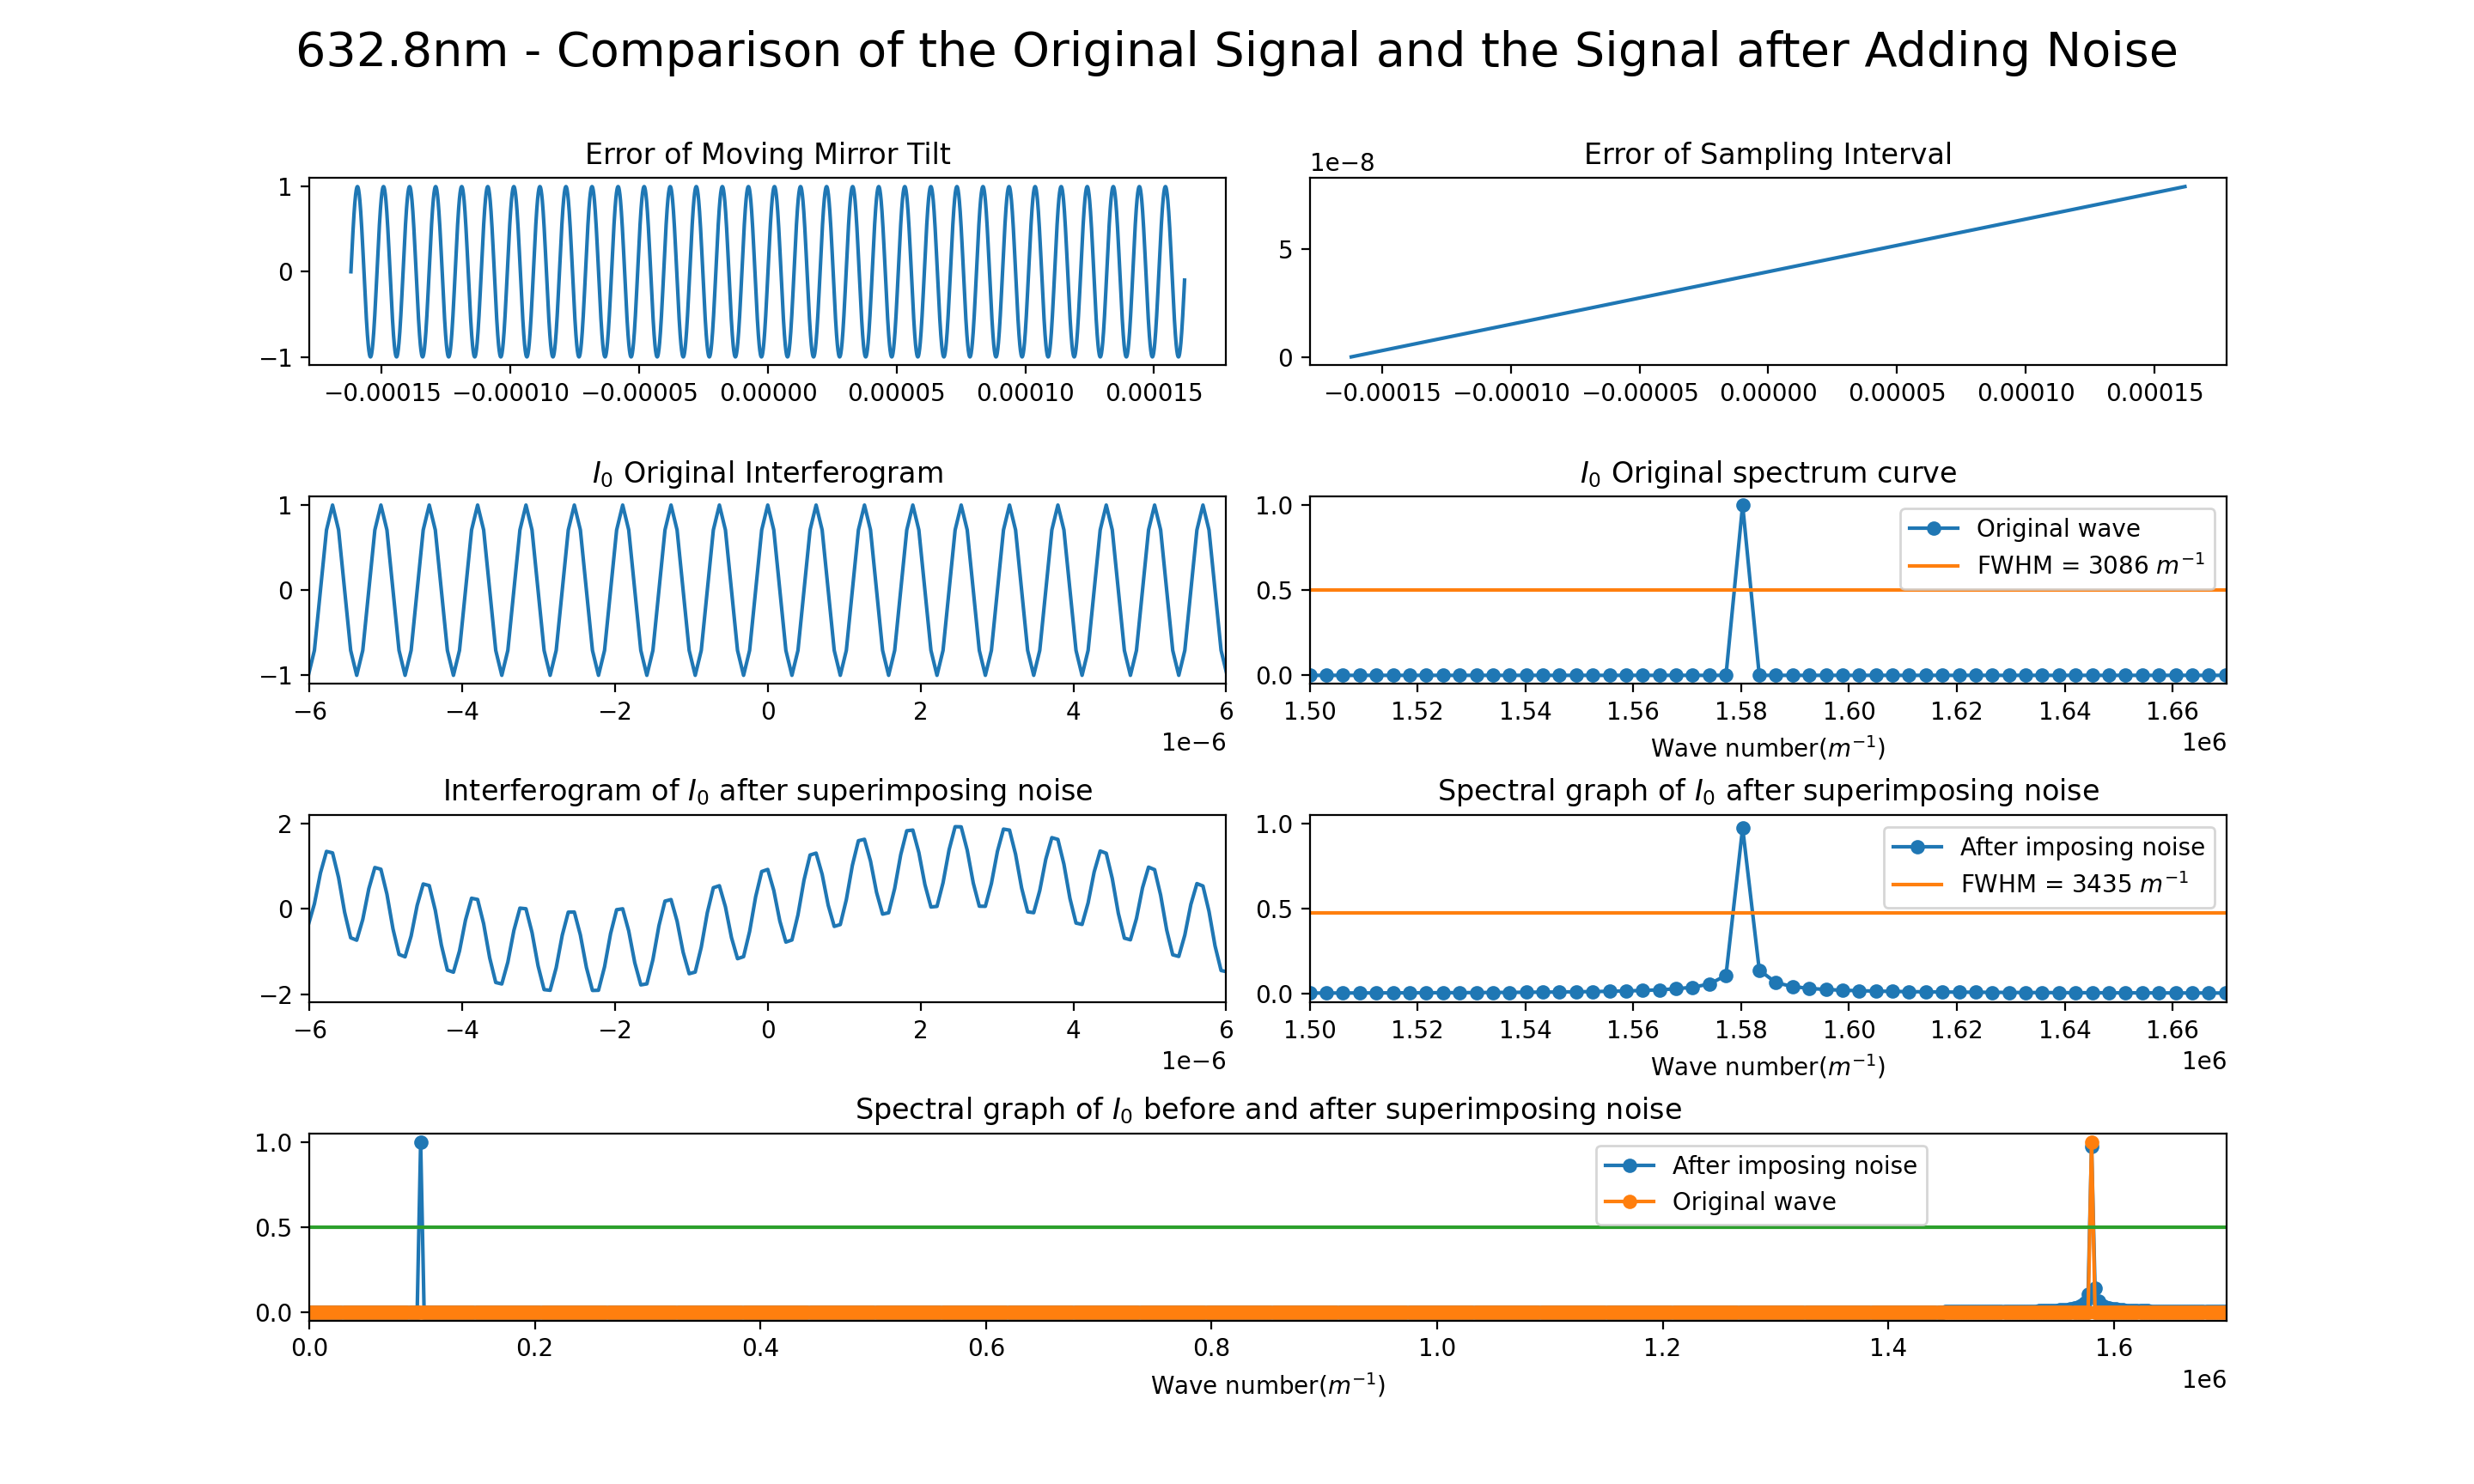
\includegraphics[width=10cm]{4.png} 	
	}
	\caption{正弦形式的动镜倾斜误差与线性形式的采样间隔误差同时作用后的傅立叶变换光谱测量曲线}
	\label{pic4}
\end{figure}

\begin{figure}[htbp]
	\centerline{
		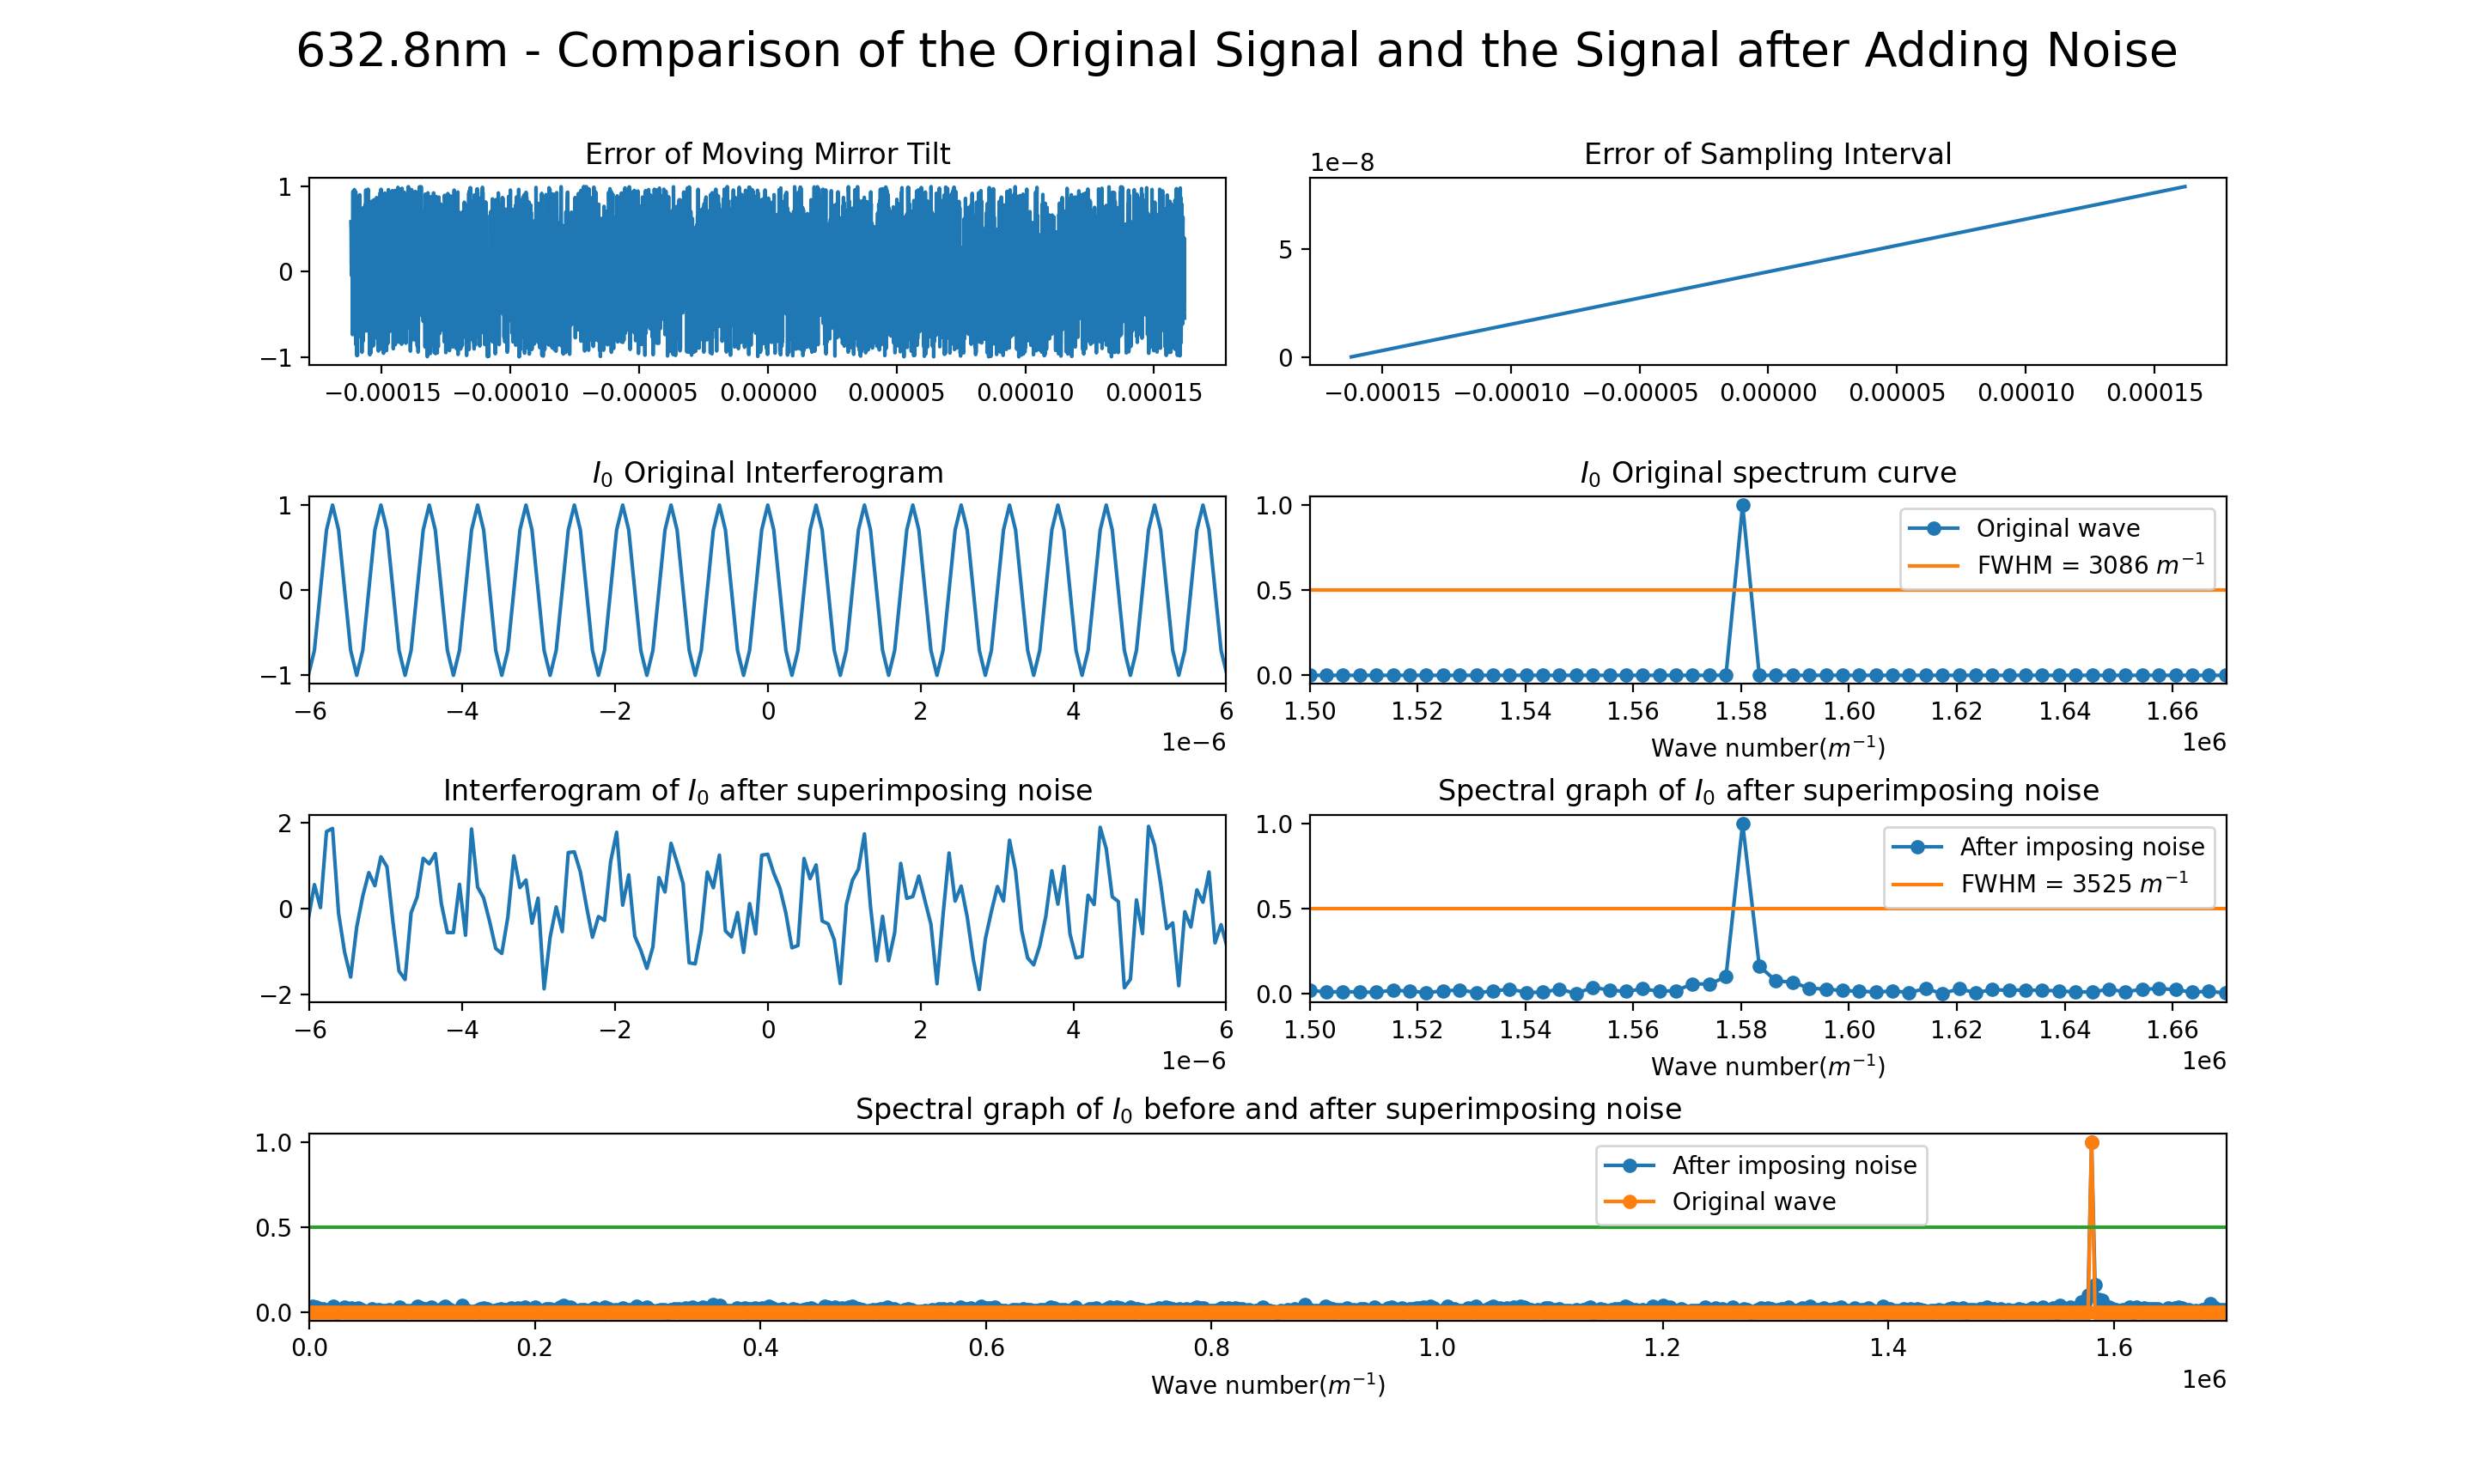
\includegraphics[width=10cm]{5.png} 	
	}
	\caption{随机形式的动镜倾斜误差与线性形式的采样间隔误差同时作用后的傅立叶变换光谱测量曲线}
	\label{pic5}
\end{figure}

\begin{figure}[htbp]
	\centerline{
		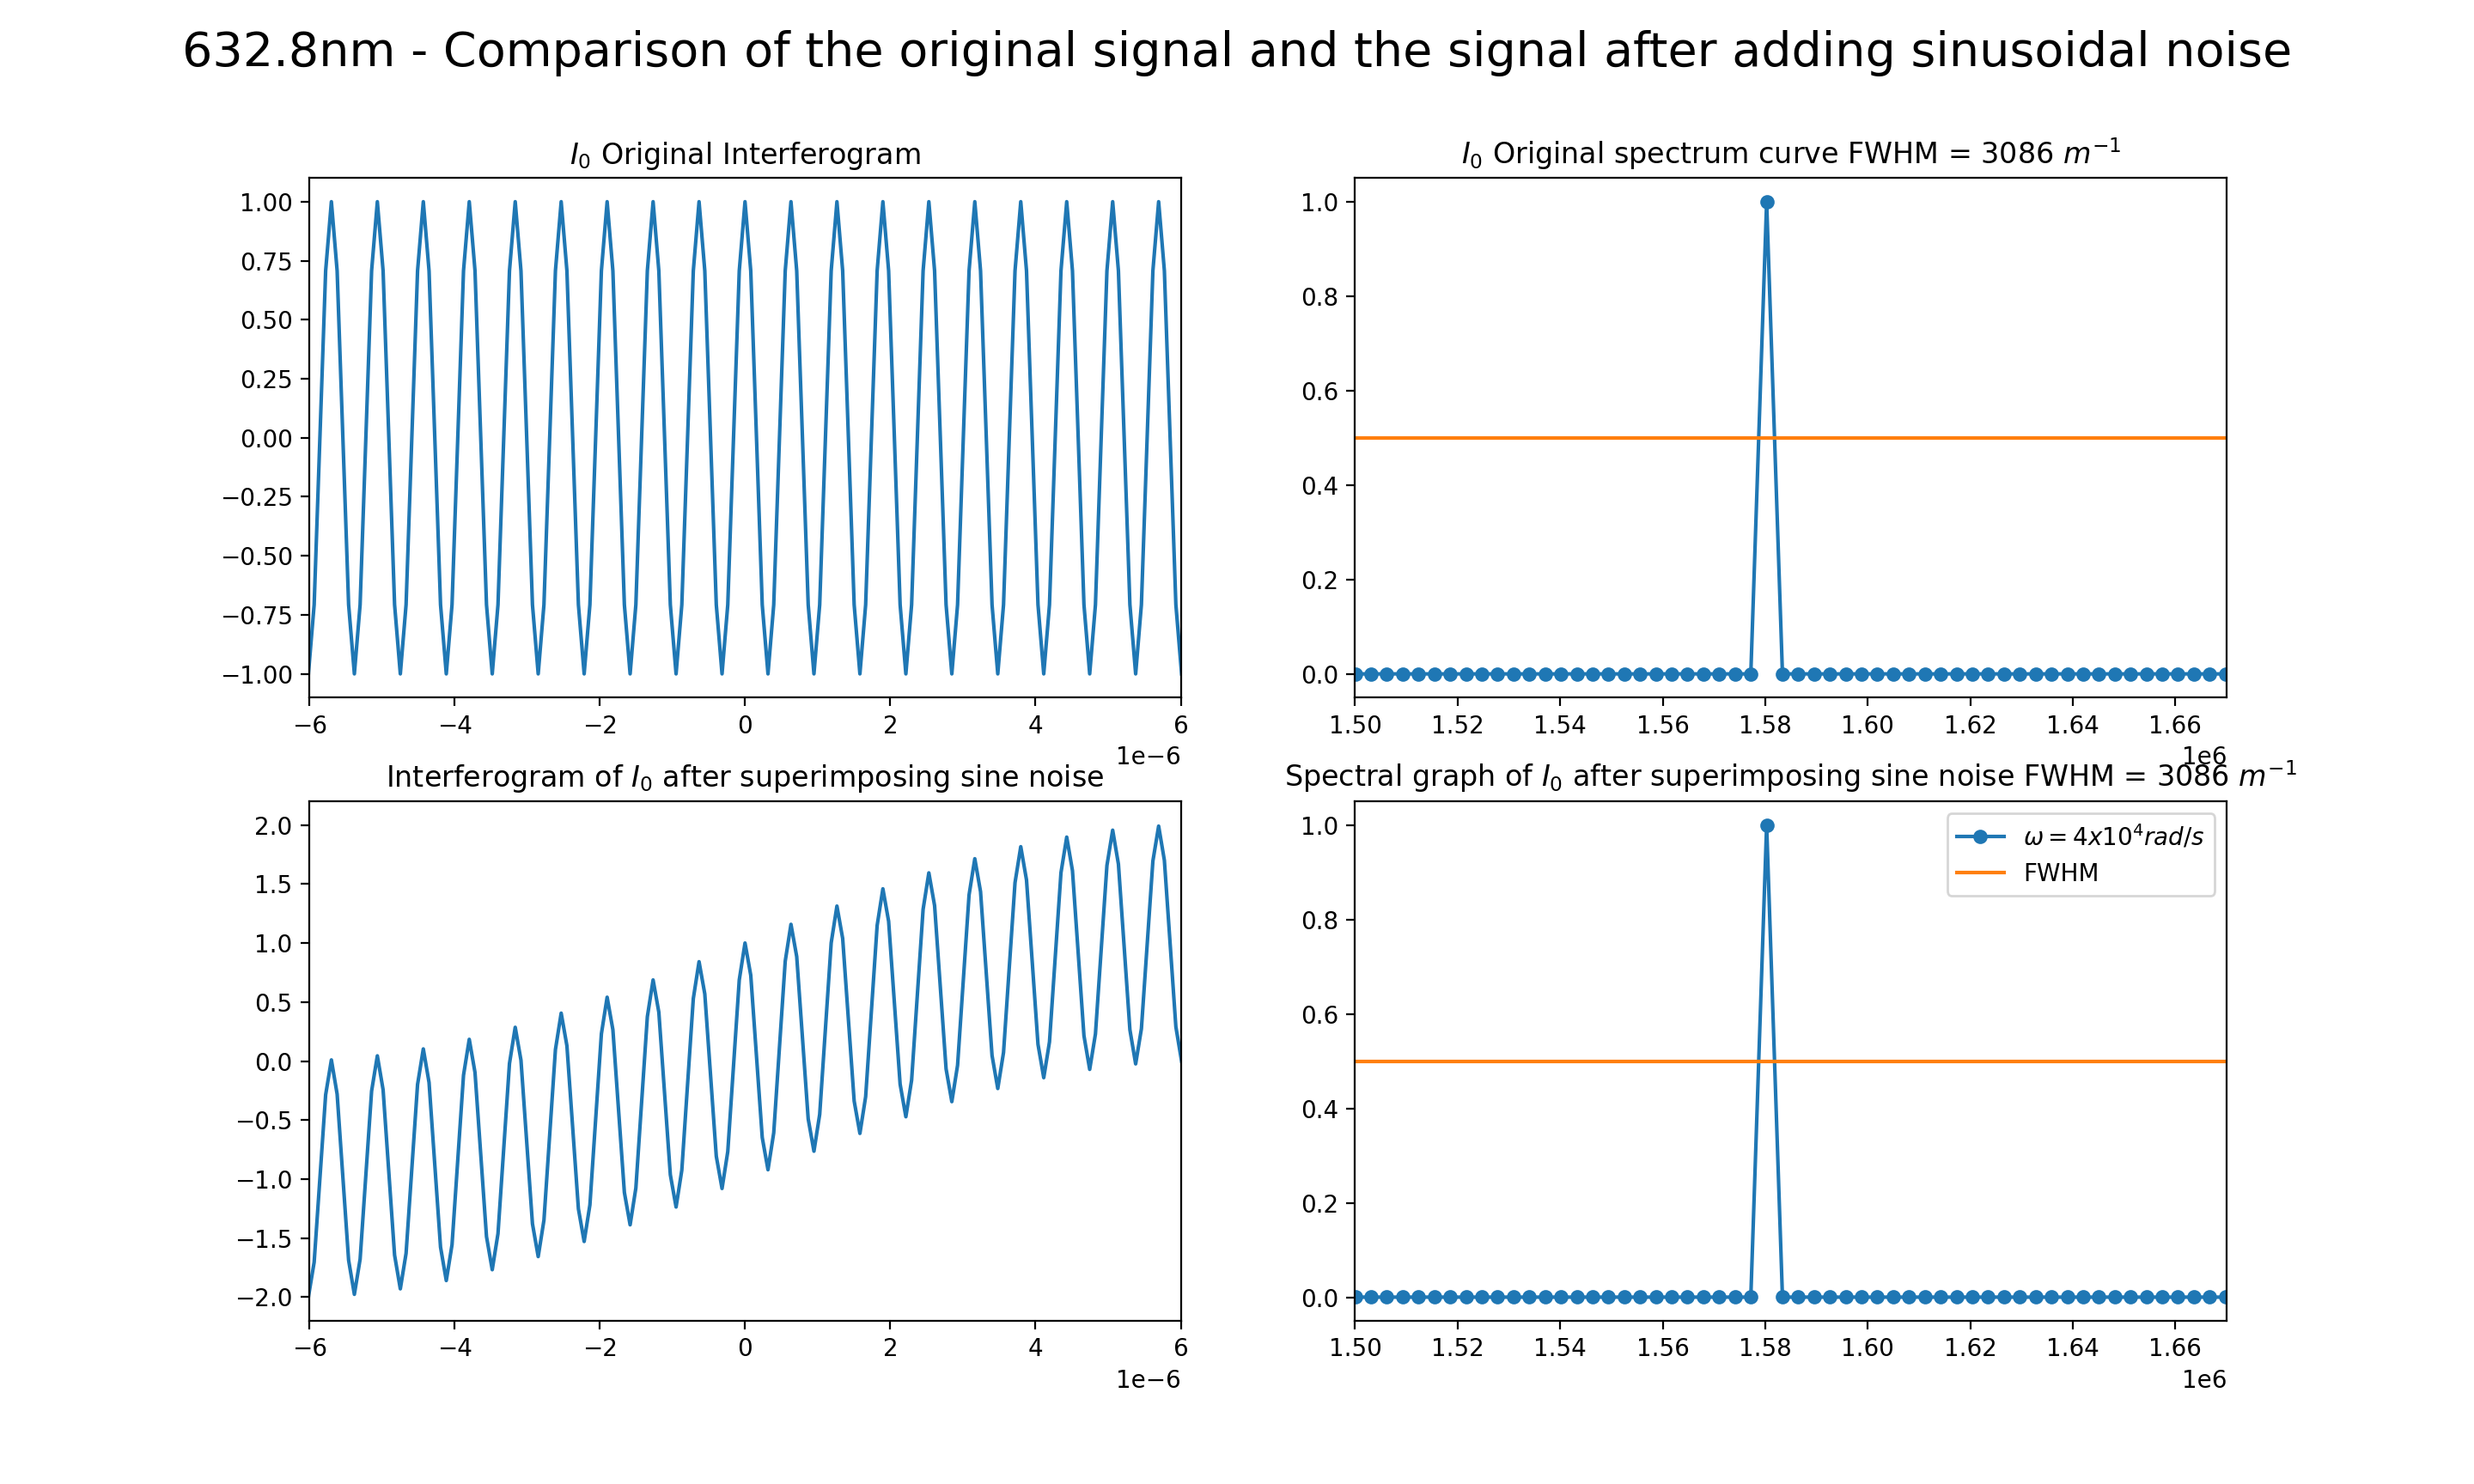
\includegraphics[width=10cm]{6.png} 	
	}
	\caption{线性形式的动镜倾斜误差与正弦形式的采样间隔误差同时作用后的傅立叶变换光谱测量曲线}
	\label{pic6}
\end{figure}

图\ref{pic4}、图\ref{pic5}与图\ref{pic6}分别显示了同时叠加动镜倾斜误差与采样间隔误差时的干涉图与傅里叶变换后的光谱测量曲线。每张图第一行表示叠加的动镜倾斜误差与采样间隔误差的类型,左半部分为动镜倾斜误差的变换曲线,右半部分为叠加的采样间隔误差。第二行表示原始未叠加动镜倾斜误差时候的干涉图与傅里叶变换光谱测量曲线。第三行展示了叠加对应的动镜倾斜误差干涉图与傅里叶变换光谱测量曲线。图片第四行为叠加动镜倾斜误差前后傅里叶变换光谱测量曲线的比较。

图\ref{pic4}显示了正弦形式的动镜倾斜误差与线性形式的采样间隔误差同时作用后的傅立叶变换光谱测量曲线结果。可以看到,叠加联合噪声后的干涉图包络按照动镜倾斜误差的形式变化。同时,叠加联合噪声后的光谱测量曲线的主峰幅度有一定的下降,主峰峰值的下降导致了主峰半峰全宽的增加,光谱测量曲线还出现了侧峰的现象。

图\ref{pic5}显示了随机形式的动镜倾斜误差与线性形式的采样间隔误差同时作用后的傅立叶变换光谱测量曲线结果。可以看到,叠加联合噪声后的干涉图包络按照动镜倾斜误差的形式变化。叠加联合噪声后的光谱测量曲线的主峰幅度没有出现峰值下降的现象,但由于存在线性形式的采样间隔误差导致了主峰半峰全宽的增加,光谱测量曲线并没有出现侧峰的现象。

图\ref{pic6}显示了线性形式的动镜倾斜误差与正弦形式的采样间隔误差同时作用后的傅立叶变换光谱测量曲线结果。可以看到,叠加联合噪声后的干涉图包络按照动镜倾斜误差的形式变化。叠加联合噪声后的光谱测量曲线的主峰幅度出现峰值下降的现象,但由于存在线性形式的动镜倾斜误差导致了主峰出现侧峰的现象,同时由于正弦形式的采样间隔误差导致了光谱测量曲线的主峰出现半峰全宽变宽的现象。

\section{结语}
本实验完成了利用Python仿真动镜倾斜误差与采样间隔误差两个因素同时影响下的傅里叶变换光谱测量系统的光谱测量曲线。

\end{document}
